\documentclass[12pt]{article}
\usepackage[letterpaper,total={6.5in,9in}]{geometry}
\usepackage{amsmath}
\usepackage{amsfonts}
\usepackage{tikz}
\usepackage{ragged2e}
\usepackage{listings}
\usepackage{setspace}
\usepackage{color}
\usepackage{multicol}
\usepackage{array}
\renewcommand{\familydefault}{\ttdefault}
\begin{document}
	\sloppy
	\begin{center}
		\huge
		\underline{Algorithms Dictionary}

		\large
		Charlie Cook -- Algorithms \& Data Structures -- 5/7/17

		\small
		Last Updated 5/9/17 -- 30 Pages -- 177 KB
	\end{center}

	\begin{center}
		\LARGE
		\underline{Trees \& Sorting}
	\end{center}

	\begin{justify}
		\large
		\underline{Binary Search Tree}

		\normalsize
		A B.S.T. is a data structure in which each element has one parent and (at most) two children; The lefthand children are always less than their parents and the righthand children are always greater than their parents. Only the location of the root/topmost element is needed to access the entire tree.

		Starting from the root, go down all the lefthand children until there are no more. The lowest lefthand child is the smallest element in the tree. From there, go back to the lowest element’s parent, then to the righthand child of said parent if it exists. Repeat until you arrive back at the root. From there, go to the first righthand child and go down it’s lefthand children until there are no more. Mirror the process described for the lefthand side of the tree, working your way down instead of up this time.

		More simply, this can be visualized as walking around the tree in a counterclockwise rotation, starting at the root. Consider elements visited only when you are below them. In the below example, when you start at 10, you are above it. You can’t be below 10 (map-wise) until you go beneath 1, 5, and 7.

		\large
		\underline{Ex.}
	\end{justify}
	\begin{center}
		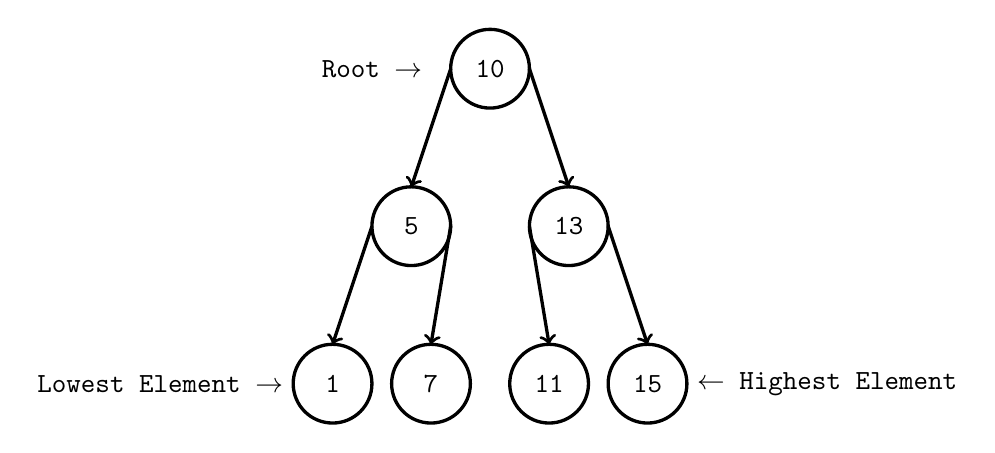
\begin{tikzpicture}
			\draw [very thick] (0,0) circle (0.5);
			\draw [very thick] (-1,-2) circle (0.5);
			\draw [very thick] (1,-2) circle (0.5);
			\draw [very thick] (-2,-4) circle (0.5);
			\draw [very thick] (-0.75,-4) circle (0.5);
			\draw [very thick] (0.75,-4) circle (0.5);
			\draw [very thick] (2,-4) circle (0.5);
			\draw [very thick, ->] (-0.5,0) -- (-1,-1.5);
			\draw [very thick, ->] (0.5,0) -- (1,-1.5);
			\draw [very thick, ->] (-1.5,-2) -- (-2,-3.5);
			\draw [very thick, ->] (-0.5,-2) -- (-0.75,-3.5);
			\draw [very thick, ->] (1.5,-2) -- (2,-3.5);
			\draw [very thick, ->] (0.5,-2) -- (0.75,-3.5);
			\node at (0,0) {10};
			\node at (-1,-2) {5};
			\node at (1,-2) {13};
			\node at (-2,-4) {1};
			\node at (-0.75,-4) {7};
			\node at (0.75,-4) {11};
			\node at (2,-4) {15};
			\node at (-1.5,0) {Root $\rightarrow$};
			\node [left] at (-2.5,-4) {Lowest Element $\rightarrow$};
			\node [right] at (2.5,-4) {$\leftarrow$ Highest Element};
		\end{tikzpicture}
	\end{center}
	\begin{justify}
		\large
		\underline{Code}

		\small
		\lstinputlisting[language=C, showstringspaces=false, firstline=5, lastline=163, breaklines=true, tabsize=2]{cc_BST.c}
	\end{justify}
	\pagebreak
	\begin{justify}
		\footnotesize
		\underline{Note: For the following five algorithms, this is the definition of the swap function:}
		\lstinputlisting[language=C, showstringspaces=false, firstline=48, lastline=52, breaklines=true, tabsize=2]{sorting.c}

		\large
		\underline{Bubble Sort}

		\normalsize
		Bubble Sort passes through an array as many times as there are elements in the array. In each pass, it checks every element against the one after it; If the after element is less than the current element, the elements are swapped. Once the last pass is complete, the array is sorted.

		Bubble Sort can be optimized to have less passes than the number of elements by adding a check; If no swaps have occurred in a pass, the array is sorted.

		\large
		\underline{Ex.}

		\small
		\begin{lstlisting}[tabsize=4]
		array (no passes):	4, 2, 1, 3		[SWAPS: 0]
		array (1 pass):		2, 1, 3, 4		[SWAPS: 3]
		array (2 passes):	1, 2, 3, 4		[SWAPS: 4]
		(The 3rd pass does not have any swaps. The list is sorted.)

		(3 passes and 4 swaps were needed.)
		\end{lstlisting}

		\large
		\underline{Code}

		\small
		\lstinputlisting[language=C, showstringspaces=false, firstline=167, lastline=189, breaklines=true, tabsize=2]{sorting.c}
	\end{justify}
	\pagebreak
	\begin{justify}
		\large
		\underline{Insertion Sort}

		\normalsize
		Insertion Sort passes through an array once, starting from the second element. Each element is inserted into its proper position. This can be done by swapping the current element and its prior element while the prior element is greater than the current element. Once the pass is done, the array is sorted.

		\large
		\underline{Ex.}

		\small
		\begin{lstlisting}[tabsize=4]
		array (no inserts):	4, 2, 1, 3
		array (1 insert):	2, 4, 1, 3
		array (2 inserts):	1, 2, 4, 3
		array (3 inserts):	1, 2, 3, 4		[SORTED]

		(1 pass and 3 swaps were needed.)
		\end{lstlisting}
		
		\large
		\underline{Code}

		\small
		\lstinputlisting[language=C, showstringspaces=false, firstline=191, lastline=207, breaklines=true, tabsize=2]{sorting.c}
	\end{justify}
	\pagebreak
	\begin{justify}
		\large
		\underline{Selection Sort}

		\normalsize
		Selection Sort passes through an array once, starting from the second element. The minimum element of all elements beyond (and including) the current element is selected and moved down the array until it is at the top of the sorted partition. The moving down is accomplished by swapping the minimum element with elements before it until it is in the sorted partition, or the element before it is smaller than the minimum. Once the pass is done, the array is sorted.

		\large
		\underline{Ex.}
		
		\small
		\begin{lstlisting}[tabsize=4]
		array (no selects):	4, 2, 1, 3
		array (1 select):	1, 4, 2, 3
		array (2 selects):	1, 2, 4, 3
		array (3 selects):	1, 2, 3, 4		[SORTED]

		(1 pass and 3 swaps were needed.)
		\end{lstlisting}
		
		\large
		\underline{Code}

		\small
		\lstinputlisting[language=C, showstringspaces=false, firstline=224, lastline=251, breaklines=true, tabsize=2]{sorting.c}
	\end{justify}
	\pagebreak
	\begin{justify}
		\large
		\underline{Merge Sort}

		\normalsize
		Merge Sort subdivides an array recursively until each partition is a single element. It then merges the one element arrays back together in order, yielding a sorted array at the end.

		\large
		\underline{Ex.}
		
		\small
		\begin{lstlisting}[tabsize=4]
		array:	4, 2, 1, 3

		part. 1:	4, 2
		subparts:	[4], [2]
		merged:	2, 4

		part. 2:	1, 3
		subparts:	[1], [3]
		merged:	1, 3
	
		merged:	1, 2, 3, 4
		\end{lstlisting}
		
		\large
		\underline{Code}

		\small
		\lstinputlisting[language=C, showstringspaces=false, firstline=253, lastline=301, breaklines=true, tabsize=2]{sorting.c}
	\end{justify}
	\pagebreak
	\begin{justify}
		\large
		\underline{Heap Sort}

		\normalsize
		Heap Sort takes the elements in an array and moves them into a heap, a tree structure where each element has at most two children. The root of the tree is the maximum element from the array, and each child is smaller than its parent. Elements in the heap can be swapped easily to keep the tree in heap form, and the maximum is always on top. To sort, simply take the root out and put it at the end of the sorted array, then reorder the heap. The heap will shrink until only one element remains.

		\large
		\underline{Ex.}
		
		\normalsize
		\begin{lstlisting}[tabsize=4]
		array (pre-heap): 	4, 2, 1, 3
		heap (0 removals):	  4		sorted array: 
							 /\
							3 1
							/
							2
		heap (1 removal):	  3		sorted array: 4
							 /\
							2 1
		heap (2 removals):	 2		sorted array: 3, 4
							 \
							 1
		heap (3 removals):	1		sorted array: 2, 3, 4
		sorted array (post-heap):	1, 2, 3, 4

		(1 heapify, 3 reorders, and 4 removals were needed.)
		\end{lstlisting}
		
		\large
		\underline{Code}

		\small
		\lstinputlisting[language=C, showstringspaces=false, firstline=342, lastline=387, breaklines=true, tabsize=2]{sorting.c}
	\end{justify}
	\pagebreak

	\begin{center}
		\LARGE
		\underline{Time Complexity}
	\end{center}

	\begin{justify}
		Time Complexity is a way to classify and rank algorithms. As the name implies, the runtime of an algorithm is what is used in ranking. An algorithm's runtime can be represented as some function of the size of the input data, commonly designated as $n$. For sorting algorithms, $n$ is the number of elements in the array that needs sorting.

		To simplify the expressions, Big-O Notation is used, which drops out the lower order terms and leading coefficient in favor of focusing on the leading term. Below is a table of time complexity classes and algorithms associated with those classes.
	\end{justify}

	\begin{center}
		\begin{tabular}{|| m{1.125in} | m{0.875in} | m{4in} ||}
			\hline
			Time Type & Big-O Type & Algorithm(s) \\
			\hline
			\hline
			Constant & $O(1)$ & Swapping Two Array Elements \\
			\hline
			Logarithmic & $O(\log{(n)})$ & Binary Search \\
			\hline
			Linear & $O(n)$ & Printing an Array, Finding Array Extrema \\
			\hline
			Linearithmic & $O(n \log{(n)})$ & Merge \& Heap Sort \\
			\hline
			Quadratic & $O(n^2)$ & Bubble, Insertion, \& Selection Sort \\
			\hline
			Factorial & $O(n!)$ & Bogo Sort (See the next page)\\
			\hline
		\end{tabular}
		\\~\\
		\large
		\underline{Time Complexity Table}
	\end{center}
	\pagebreak

	\begin{center}
		\LARGE
		\underline{The Traveling Salesman Problem}
	\end{center}

	\begin{justify}
		The Traveling Salesman Problem is an open NP-Hard problem in Computer Science. It simply states:
		\\~\\
		\textsf{Given a list of cities and the distances between them, what is the shortest route that will let you visit all cities and return to the city you start from?}
		\\~\\
		An alternate version of it, designated the T.S.P. Decision Version, also exists, which states:
		\\~\\
		\textsf{Given a limit to the distance of a route, does a viable route exist that will satisfy T.S.P. and be under the limit?}
		\\~\\
		If we reference the graph below, say we want to start from Fitchburg (node 3) and visit all of the eight cities in the New England area that are shown. If we consider the normal version of T.S.P., the first thing we might try is to list out all routes that visit all cities and end up back in Fitchburg. This might take a while, and if we also wanted to visit some small towns as well, say we add 20 of them to the graph, the number of routes will grow worse than exponentially.

		In fact, attempting this method of brute-forcing T.S.P. has a time complexity of $O(n!)$, where $n$ is the number of cities. Bogo Sort also has this time complexity. For those unaware, Bogo Sort involves randomly shuffling a list, checking if its sorted, and repeating until the list is sorted. Clearly, brute-force will not be efficient for this problem, hence it's classification as NP-Hard.
	\end{justify}

	\begin{center}
		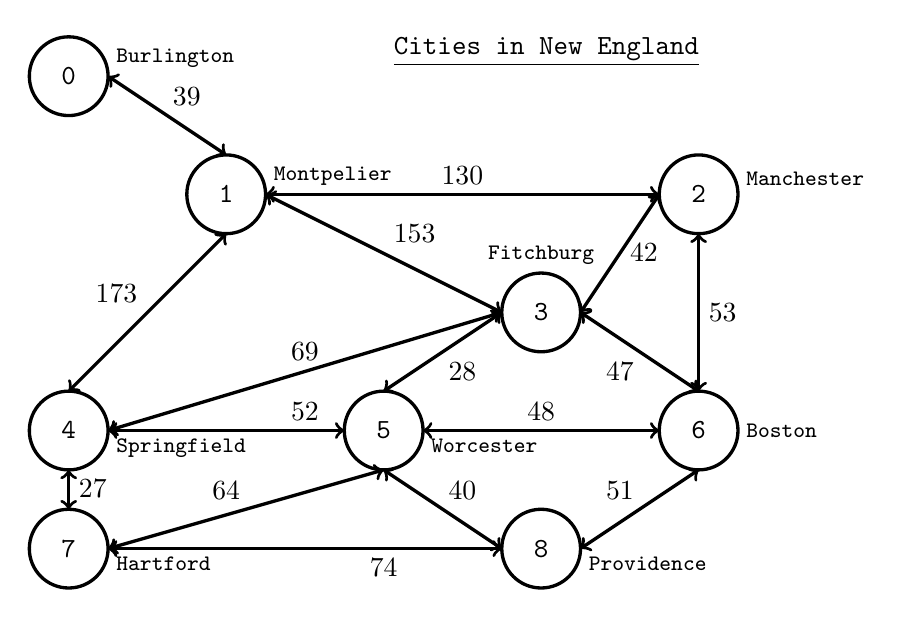
\begin{tikzpicture}
			\draw [very thick] (-4,6) circle (0.5);
			\draw [very thick] (-2,4.5) circle (0.5);
			\draw [very thick] (4,4.5) circle (0.5);
			\draw [very thick] (2,3) circle (0.5);
			\draw [very thick] (-4,1.5) circle (0.5);
			\draw [very thick] (0,1.5) circle (0.5);
			\draw [very thick] (4,1.5) circle (0.5);
			\draw [very thick] (-4,0) circle (0.5);
			\draw [very thick] (2,0) circle (0.5);
			\normalsize
			\node at (-4,6) {0};
			\node at (-2,4.5) {1};
			\node at (4,4.5) {2};
			\node at (2,3) {3};
			\node at (-4,1.5) {4};
			\node at (0,1.5) {5};
			\node at (4,1.5) {6};
			\node at (-4,0) {7};
			\node at (2,0) {8};
			\footnotesize
			\node [above right] at (-3.5,6) {Burlington};
			\node [above right] at (-1.5,4.5) {Montpelier};
			\node [above right] at (4.5,4.5) {Manchester};
			\node [above] at (2,3.5) {Fitchburg};
			\node [below right] at (-3.5,1.5) {Springfield};
			\node [below right] at (0.5,1.5) {Worcester};
			\node [right] at (4.5,1.5) {Boston};
			\node [below right] at (-3.5,0) {Hartford};
			\node [below right] at (2.5,0) {Providence};

			\draw [very thick, <->] (-3.5,6) -- (-2,5);
			\draw [very thick, <->] (-2,4) -- (-4,2);
			\draw [very thick, <->] (-1.5,4.5) -- (3.5,4.5);
			\draw [very thick, <->] (-1.5,4.5) -- (1.5,3);
			\draw [very thick, <->] (3.5,4.5) -- (2.5,3);
			\draw [very thick, <->] (4,4) -- (4,2);
			\draw [very thick, <->] (2.5,3) -- (4,2);
			\draw [very thick, <->] (1.5,3) -- (0,2);
			\draw [very thick, <->] (1.5,3) -- (-3.5,1.5);
			\draw [very thick, <->] (-3.5,1.5) -- (-0.5,1.5);
			\draw [very thick, <->] (0.5,1.5) -- (3.5,1.5);
			\draw [very thick, <->] (-4,1) -- (-4,0.5);
			\draw [very thick, <->] (0,1) -- (-3.5,0);
			\draw [very thick, <->] (0,1) -- (1.5,0);
			\draw [very thick, <->] (-3.5,0) -- (1.5,0);
			\draw [very thick, <->] (2.5,0) -- (4,1);
			\normalsize
			\node [above] at (-2.5,5.5) {$39$};
			\node [above] at (1,4.5) {$130$};
			\node [right] at (4,3) {$53$};
			\node [right] at (0,4) {$153$};
			\node [above left] at (-3,3) {$173$};
			\node at (-1,2.5) {$69$};
			\node [above] at (1,2) {$28$};
			\node [above] at (3,2) {$47$};
			\node [below right] at (3,4) {$42$};
			\node [above] at (-1,1.5) {$52$};
			\node [above] at (2,1.5) {$48$};
			\node [below right] at (-4,1) {$27$};
			\node [below] at (0,0) {$74$};
			\node [above] at (-2,0.5) {$64$};
			\node [above] at (1,0.5) {$40$};
			\node [above] at (3,0.5) {$51$};
			\node [above right] at (0,6) {\underline{Cities in New England}};
		\end{tikzpicture}
	\end{center}
	\pagebreak

	\begin{center}
		\LARGE
		\underline{Dijkstra \& Pathfinding}
	\end{center}

	\begin{justify}
		Dijkstra's Shortest Path Algorithm is fairly straightforward. First, you need a graph/map, which consists of a group of nodes linked in a certain fashion. The nodes should be numbered starting from 0, and can be represented as a square matrix or two-dimensional array. In this, a row corresponds to the paths that lead out of a node, and a column corresponds to the paths that lead into a node.

		To find the shortest path through the graph or from a given node to every other, do the following:
		\begin{enumerate}
			\item Create three arrays as long as the number of nodes in the graph. Name them "distance", "accessed", and "previous"
			\item Initialize the distance and previous arrays to be all -1, except the index corresponding the the origin node. For that node, set its distance to 0 and previous to its index in the matrix
			\item Initialize the accessed array be all 0, except the origin node, which should be 1.
			\item From the origin node, scan through its row in the matrix. If the distance to a new node plus the distance to the origin node is less than the current distance to the new node, or there is a path to the new node and no path to it currently exists (i.e. it has a distance value of -1), update the distance to the new node and its entry in the previous array.
			\item Once the row of the origin node is scanned, select the node that has the smallest distance and is also unaccessed. Move to this node, and set it as accessed.
			\item Repeat steps 4 and 5 until all nodes have been accessed. The final versions of the distance and previous arrays will allow you to extrapolate the shortest paths to any node.
		\end{enumerate}

		To read a path to a node, go to its entry in the previous array. Read what node was prior to your target node, and check its prior node. Repeat this until you find a node who is its own prior node, which corresponds to the origin node. Then, start printing the indicies of the nodes from origin to target.

		\pagebreak
		\large
		\underline{Ex.}

		\begin{center}
			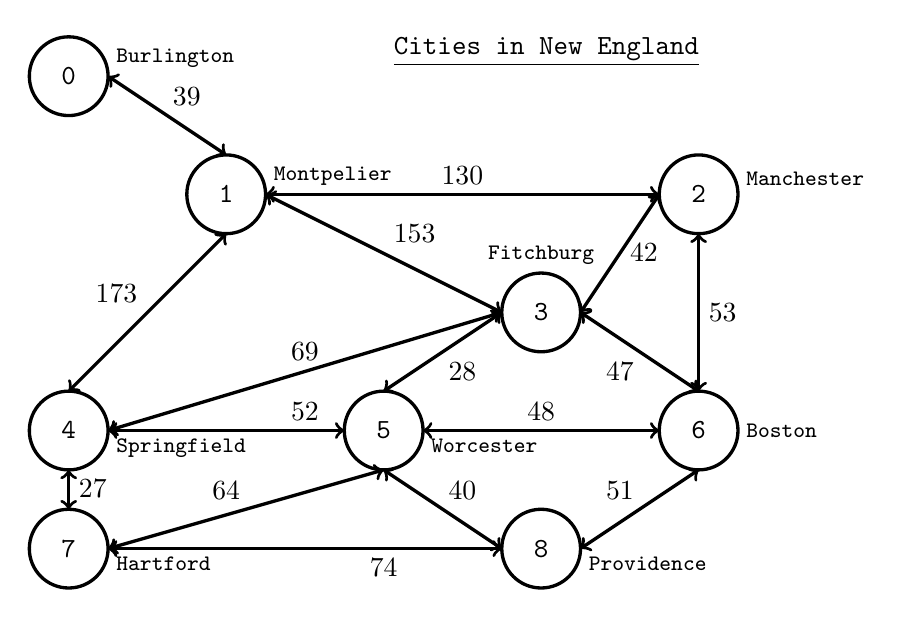
\begin{tikzpicture}
				\draw [very thick] (-4,6) circle (0.5);
				\draw [very thick] (-2,4.5) circle (0.5);
				\draw [very thick] (4,4.5) circle (0.5);
				\draw [very thick] (2,3) circle (0.5);
				\draw [very thick] (-4,1.5) circle (0.5);
				\draw [very thick] (0,1.5) circle (0.5);
				\draw [very thick] (4,1.5) circle (0.5);
				\draw [very thick] (-4,0) circle (0.5);
				\draw [very thick] (2,0) circle (0.5);
				\normalsize
				\node at (-4,6) {0};
				\node at (-2,4.5) {1};
				\node at (4,4.5) {2};
				\node at (2,3) {3};
				\node at (-4,1.5) {4};
				\node at (0,1.5) {5};
				\node at (4,1.5) {6};
				\node at (-4,0) {7};
				\node at (2,0) {8};
				\footnotesize
				\node [above right] at (-3.5,6) {Burlington};
				\node [above right] at (-1.5,4.5) {Montpelier};
				\node [above right] at (4.5,4.5) {Manchester};
				\node [above] at (2,3.5) {Fitchburg};
				\node [below right] at (-3.5,1.5) {Springfield};
				\node [below right] at (0.5,1.5) {Worcester};
				\node [right] at (4.5,1.5) {Boston};
				\node [below right] at (-3.5,0) {Hartford};
				\node [below right] at (2.5,0) {Providence};

				\draw [very thick, <->] (-3.5,6) -- (-2,5);
				\draw [very thick, <->] (-2,4) -- (-4,2);
				\draw [very thick, <->] (-1.5,4.5) -- (3.5,4.5);
				\draw [very thick, <->] (-1.5,4.5) -- (1.5,3);
				\draw [very thick, <->] (3.5,4.5) -- (2.5,3);
				\draw [very thick, <->] (4,4) -- (4,2);
				\draw [very thick, <->] (2.5,3) -- (4,2);
				\draw [very thick, <->] (1.5,3) -- (0,2);
				\draw [very thick, <->] (1.5,3) -- (-3.5,1.5);
				\draw [very thick, <->] (-3.5,1.5) -- (-0.5,1.5);
				\draw [very thick, <->] (0.5,1.5) -- (3.5,1.5);
				\draw [very thick, <->] (-4,1) -- (-4,0.5);
				\draw [very thick, <->] (0,1) -- (-3.5,0);
				\draw [very thick, <->] (0,1) -- (1.5,0);
				\draw [very thick, <->] (-3.5,0) -- (1.5,0);
				\draw [very thick, <->] (2.5,0) -- (4,1);
				\normalsize
				\node [above] at (-2.5,5.5) {$39$};
				\node [above] at (1,4.5) {$130$};
				\node [right] at (4,3) {$53$};
				\node [right] at (0,4) {$153$};
				\node [above left] at (-3,3) {$173$};
				\node at (-1,2.5) {$69$};
				\node [above] at (1,2) {$28$};
				\node [above] at (3,2) {$47$};
				\node [below right] at (3,4) {$42$};
				\node [above] at (-1,1.5) {$52$};
				\node [above] at (2,1.5) {$48$};
				\node [below right] at (-4,1) {$27$};
				\node [below] at (0,0) {$74$};
				\node [above] at (-2,0.5) {$64$};
				\node [above] at (1,0.5) {$40$};
				\node [above] at (3,0.5) {$51$};
				\node [above right] at (0,6) {\underline{Cities in New England}};
			\end{tikzpicture}
		\end{center}

		\normalsize (NE.txt)
		\small
		\lstinputlisting[tabsize=4]{NE.txt}

		\normalsize (NE\_Solved.txt)
		\footnotesize
		\lstinputlisting[tabsize=8]{NE_Solved.txt}

		\pagebreak
		\large
		\underline{Code}

		\small
		\lstinputlisting[language=C, showstringspaces=false, breaklines=true, tabsize=2]{cc_Dijkstra.c}
	\end{justify}
	\pagebreak

	\begin{center}
		\LARGE
		\underline{Theory of Computation}
	\end{center}

	\begin{center}
		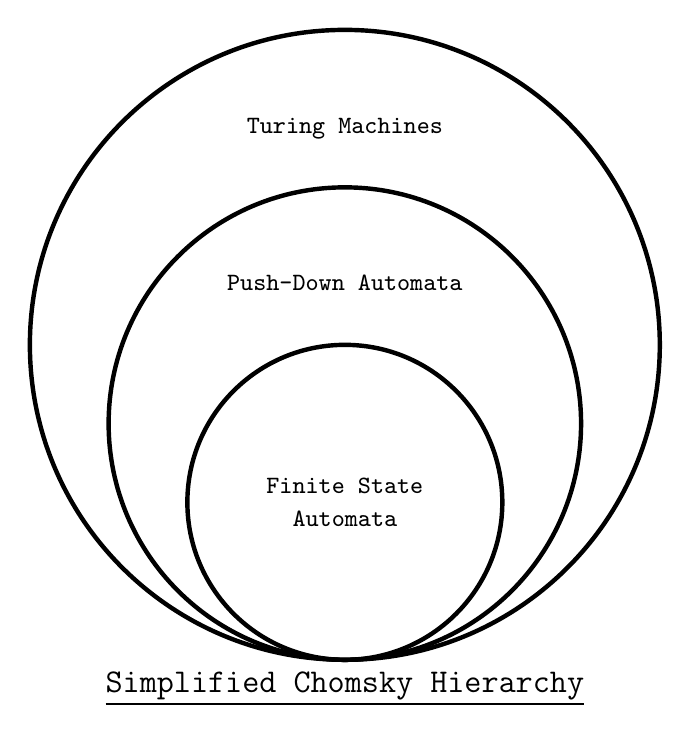
\begin{tikzpicture}
			\large
			\node [below] at (0,0) {\underline{Simplified Chomsky Hierarchy}};
			\draw [ultra thick] (0,2) circle (2);
			\draw [ultra thick] (0,3) circle (3);
			\draw [ultra thick] (0,4) circle (4);
			\small
			\node [above] at (0,2) {Finite State};
			\node [below] at (0,2) {Automata};
			\node [below] at (0,5) {Push-Down Automata};
			\node [below] at (0,7) {Turing Machines};
		\end{tikzpicture}
	\end{center}

	\begin{justify}
		\large
		\underline{Finite State Automata}

		\normalsize
		Finite State Automata, found in the center of Chomsky's Hierarchy (pictured above), are the simplest forms of computers. They can be visualized as a graph of nodes, where the start node has a blank arrow leading into it and where the end node is a double-circle. For example, below is a F.S.T. that can generate all strings that have an even number of 0's followed by an odd number of 1's. Please note that arrows marked with a $\lambda$ are null paths, which do not produce anything.
	\end{justify}

	\begin{center}
		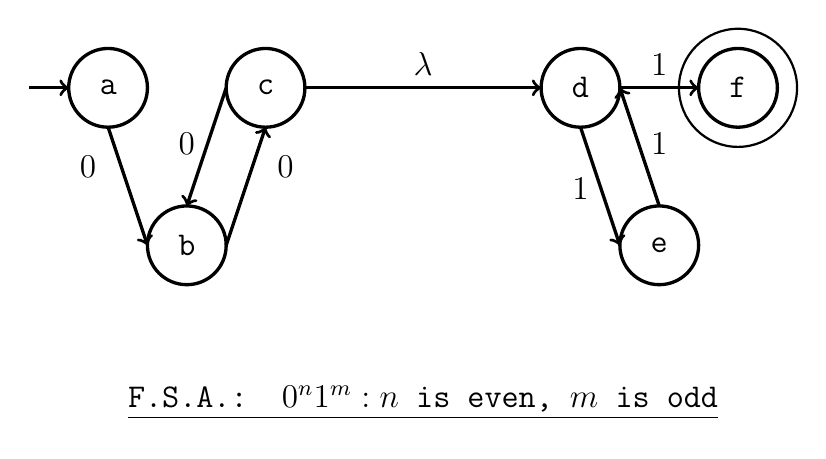
\begin{tikzpicture}
			\large
			\node at (0,0) {\underline{F.S.A.: $0^n1^m:n$ is even, $m$ is odd}};
			\draw [very thick] (-4,4) circle (0.5);
			\draw [very thick] (-2,4) circle (0.5);
			\draw [very thick] (-3,2) circle (0.5);
			\draw [very thick] (2,4) circle (0.5);
			\draw [very thick] (4,4) circle (0.5);
			\draw [very thick] (3,2) circle (0.5);
			\draw [thick] (4,4) circle (0.75);
			\node at (-4,4) {a};
			\node at (-2,4) {c};
			\node at (-3,2) {b};
			\node at (2,4) {d};
			\node at (4,4) {f};
			\node at (3,2) {e};
			\draw [very thick, ->] (-5,4) -- (-4.5,4);
			\draw [very thick, ->] (-4,3.5) -- (-3.5,2);
			\draw [very thick, ->] (-2.5,2) -- (-2,3.5);
			\draw [very thick, ->] (-1.5,4) -- (1.5,4);
			\draw [very thick, ->] (2.5,4) -- (3.5,4);
			\draw [very thick, ->] (3,2.5) -- (2.5,4);
			\draw [very thick, ->] (2,3.5) -- (2.5,2);
			\draw [very thick, ->] (-2.5,4) -- (-3,2.5);
			\node [above] at (0,4) {$\lambda$};
			\node [left] at (-4,3) {$0$};
			\node [right] at (-2,3) {$0$};
			\node [above] at (-3,3) {$0$};
			\node [below] at (2,3) {$1$};
			\node [above] at (3,3) {$1$};
			\node [above] at (3,4) {$1$};
		\end{tikzpicture}
	\end{center}
	\pagebreak

	\begin{justify}
		\large
		\underline{Push-Down Automata}

		\normalsize
		Push-Down Automata, which encompass Finite State Automata, implement a stack as a crude form of memory. The concept of a stack is critical to Computer Science, as it can represent recursion and other tricky concepts in an elementary way. A stack can have objects pushed onto it or popped off of it. Only the top element on a stack, the element last pushed on, can be popped off. Though physical implementations of stacks generally have a limit to their size, for our purposes, assume stacks can fit near-infinitely many elements.

		One thing that Push-Down Automata can do that Finite State Automata cannot is generate all strings that have an equal number of 0's and 1's. Also, Push-Down Automata can generate all binary palindrome strings. Examples of both of these can be seen below. It should be noted that in order for an automata to finish, its stack must be empty. Also, if a push invovles a letter, that letter must be at the top of the stack in order for a pull of it to be processed. Finally, as with Finite State Automata, $\lambda$ paths do not do anything.
	\end{justify}

	\begin{multicols}{2} \begin{center}
		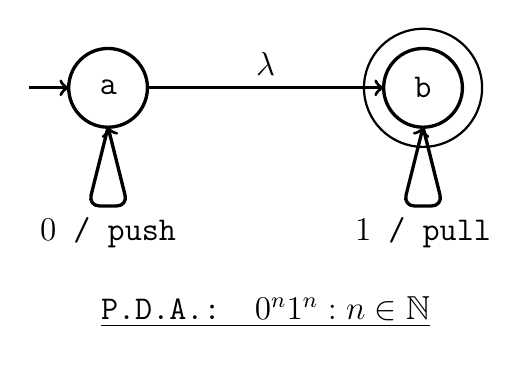
\begin{tikzpicture}
			\large
			\node [below] at (0,-0.5) {\underline{P.D.A.: $0^n1^n : n \in \mathbb{N}$}};
			\draw [very thick] (-2,2) circle (0.5);
			\draw [very thick] (2,2) circle (0.5);
			\draw [thick] (2,2) circle (0.75);
			\draw [very thick, rounded corners, ->] (-2,1.5) -- (-2.25,0.5) -- (-1.75,0.5) -- (-2,1.5);
			\draw [very thick, rounded corners, ->] (2,1.5) -- (2.25,0.5) -- (1.75,0.5) -- (2,1.5);
			\draw [very thick, ->] (-1.5,2) -- (1.5,2);
			\draw [very thick, ->] (-3,2) -- (-2.5,2);
			\node at (-2,2) {a};
			\node at (2,2) {b};
			\node [below] at (-2,0.5) {$0$ / push};
			\node [below] at (2,0.5) {$1$ / pull};
			\node [above] at (0,2) {$\lambda$};
		\end{tikzpicture}
		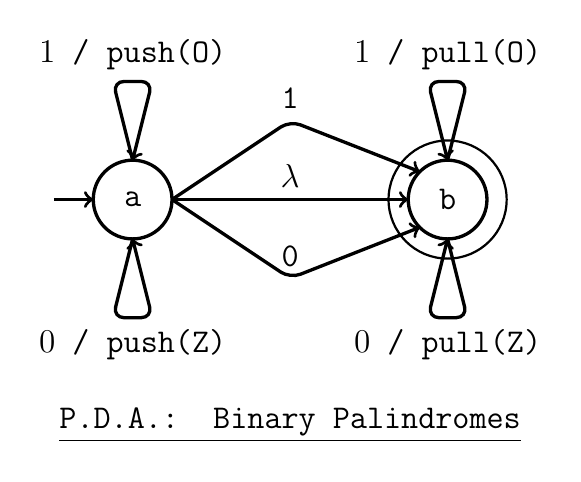
\begin{tikzpicture}
			\large
			\node [below] at (0,-0.5) {\underline{P.D.A.: Binary Palindromes}};
			\draw [very thick] (-2,2) circle (0.5);
			\draw [very thick] (2,2) circle (0.5);
			\draw [thick] (2,2) circle (0.75);
			\draw [very thick, rounded corners, ->] (-2,1.5) -- (-2.25,0.5) -- (-1.75,0.5) -- (-2,1.5);
			\draw [very thick, rounded corners, ->] (2,1.5) -- (2.25,0.5) -- (1.75,0.5) -- (2,1.5);
			\draw [very thick, rounded corners, ->] (-2,2.5) -- (-2.25,3.5) -- (-1.75,3.5) -- (-2,2.5);
			\draw [very thick, rounded corners, ->] (2,2.5) -- (2.25,3.5) -- (1.75,3.5) -- (2,2.5);
			\draw [very thick, ->] (-1.5,2) -- (1.5,2);
			\draw [very thick, ->] (-3,2) -- (-2.5,2);
			\draw [very thick, rounded corners, ->] (-1.5,2) -- (0,3) -- (1.647,2.354);
			\draw [very thick, rounded corners, ->] (-1.5,2) -- (0,1) -- (1.647,1.647);
			\node at (-2,2) {a};
			\node at (2,2) {b};
			\node [below] at (-2,0.5) {$0$ / push(Z)};
			\node [below] at (2,0.5) {$0$ / pull(Z)};
			\node [above] at (0,2) {$\lambda$};
			\node [above] at (0,3) {1};
			\node [above] at (0,1) {0};
			\node [above] at (-2,3.5) {$1$ / push(O)};
			\node [above] at (2,3.5) {$1$ / pull(O)};
		\end{tikzpicture}
	\end{center} \end{multicols}
	\pagebreak
	
	\begin{justify}
		\large
		\underline{Turing Machines}

		\normalsize
		Turing Machines, which encompass the prior two automata types, can compute the answer to any problem for which an algorithm exists. Pioneered and commemorated to Alan Turing, the Father of Computer Science, they function as such:

		Using a (reasonably) infitine tape of cells, a Turing Machine is instructed with a set of rules. For each rule, the T.M. reads the current cell it is at on the tape. Based on what is read, the T.M. may change to a new state, and may overwrite the cell. Once a state-change and/or a write occur, the T.M. will then move one cell to the left or to the right. Eventually, a properly designed Turing Machine will enter a halt state, in which it can be in an "accept" substate, or in a "reject" substate.

		The concept of the state, coupled with the tape of data and instructions, paved the way for the development of general purpose computers following the Second World War in the mid 20th Century. Unfortunately, due to homophobic sentiments and nosy police officers, Alan Turing was forced into hormone theropy when it was revealed he was gay, a crime under contemporary British law. This, coupled with the resentment Turing now faced in the industry, led him to end his life prematurely, and he would not be pardoned by the government of Britain for nearly five decades afterwards. Back on topic.

		Below are instructions for a Turing Machine that will increment a binary number on a tape. Each instruction should be read as:

		\begin{center}
			\small
			[Current State], [Data Read]=>[New State], [Data Write], [Move Tape]
		\end{center}

		S is the starting state. $\delta$ is the leftmost cell on the tape, and beyond which the machine is barred from going. \_ is a blank cell. Once the "accept" state is entered, the machine halts.
	\end{justify}

	\begin{multicols}{3}
		\begin{lstlisting}[tabsize=6, escapeinside={(*}{*)}]
S, (*$\delta$*)=>S, (*$\delta$*), R;
S, 0=>Z, 0, R;
S, 1=>(*$\Omega$*), 1, R;


(*$\Omega$*), 1=>(*$\Omega$*), 1, R;
(*$\Omega$*), 0=>Z, 0, R;
(*$\Omega$*), _=>F, 0, L;
		\end{lstlisting}
		\begin{lstlisting}[tabsize=6, escapeinside={(*}{*)}]
Z, 0=>Z, 0, R;
Z, 1=>Z, 1, R;
Z, _=>A, _, L;



A, 0=>H, 1, L;
A, 1=>A, 0, L;
		\end{lstlisting}
		\begin{lstlisting}[tabsize=6, escapeinside={(*}{*)}]
H, 0=>H, 0, L;
H, 1=>H, 1, L;
H, (*$\delta$*)=>accept;

F, 1=>F, 0, L;
F, (*$\delta$*)=>W, (*$\delta$*), R;

W, 0=>H, 1, L;
		\end{lstlisting}
	\end{multicols}

	\begin{center}
		\large
		\underline{T.M.: Binary Incrementer with Overflow Accommodation}
	\end{center}
	\pagebreak

	\begin{center}
		\LARGE
		\underline{RSA Encryption}
	\end{center}

	\begin{center}
		\small
		Note: the traditional Alice and Bob characters will be supplemented by \textcolor{blue}{Amuro Ray} and \textcolor{yellow}{Sayla Mass} from Mobile Suit Gundam.
	\end{center}

	\begin{FlushLeft}
		\textcolor{blue}{Amuro} and \textcolor{yellow}{Sayla} wish to talk securely, since they know \textcolor{red}{Char}, \textcolor{yellow}{Sayla}'s over-protective and slightly fascist older brother, is listening to them. First, they each pick two prime numbers (usually large but for this example they will be small) to keep secret.
		\\~\\
		\textcolor{blue}{Amuro}'s primes, $P_A$ and $Q_A$, are $5$ and $29$.

		\textcolor{yellow}{Sayla}'s primes, $P_S$ and $Q_S$, are $7$ and $23$.
		\\~\\
		\textcolor{blue}{Amuro} transmits the product of his primes, $N_A = 145 (= 5 * 29)$.

		\textcolor{yellow}{Sayla} transmits the product of her primes, $N_S = 161 (= 7 * 23)$.
		\\~\\
		\textcolor{red}{Char} can see both $N_A$ and $N_S$. So too can \textcolor{yellow}{Sayla} and \textcolor{blue}{Amuro}.
		\\~\\
		\textcolor{blue}{Amuro} picks another prime number, $E_A = 13$, and transmits it.

		\textcolor{yellow}{Sayla} picks another prime number, $E_S = 17$, and transmits it.
		\\~\\
		\textcolor{red}{Char} can see both $E_A$ and $E_S$. So too can \textcolor{yellow}{Sayla} and \textcolor{blue}{Amuro}. $E_A$ and $E_S$ act as \textcolor{blue}{Amuro} and \textcolor{yellow}{Sayla}'s public/encryption keys. Now \textcolor{blue}{Amuro} and \textcolor{yellow}{Sayla} can send each other encrypted messages.
		\\~\\
		Using ASCII, \textcolor{blue}{Amuro} encrypts his message, $M_A$ = "X", or $88$ in ASCII, using the following formula:

		\begin{center}
			${M_A}^{E_S} \mod N_S = 88^{17} \mod 161 = 44 =$ "," $= C_A$
		\end{center}

		$C_A$ is \textcolor{blue}{Amuro}'s ciphertext, which he can transmit. He does.
		\\~\\
		\textcolor{yellow}{Sayla} chooses her message, $M_S = $ "O", or $79$ in ASCII, and uses a similar formula:

		\begin{center}
			${M_S}^{E_A} \mod N_A = 79^{13} \mod 145= 69 =$ "E" $= C_S$
		\end{center}

		$C_S$ is \textcolor{yellow}{Sayla}'s ciphertext, which she can transmit. She does.
		\\~\\
		\textcolor{red}{Char} can see \textcolor{blue}{Amuro} and \textcolor{yellow}{Sayla}'s ciphertexts, "," and "E", and is perplexed.
	\end{FlushLeft}
	\pagebreak
	\begin{FlushLeft}
		To decrypt $C_S$, \textcolor{blue}{Amuro} must calculate his private/decryption key, $D_A$. He can do this because of the following congruence:
		
		\begin{center}
		$E_A * D_A \equiv 1 \mod (P_A -1) * (Q_A - 1)$
		\end{center}

		This translates to the equation:

		\begin{center}
		$E_A * D_A = k * (P_A -1) * (Q_A - 1) + 1$
		\end{center}

		Where $k$ is some integer. Solving this equation for $D_A$ shows:
		\begin{align*}
			D_A &= (k * (P_A -1) * (Q_A - 1) + 1) / E_A \\
				&= (k * (5 -1) * (29 - 1) + 1) / 13 \\
				&= (k * 4 * 28 + 1) / 13 \\
				&= (112k + 1) / 13
		\end{align*}

		$D_A$ needs to be an integer, and $k = 8$ results in $D_A = 69$.
		\\~\\
		\textcolor{blue}{Amuro} can put $C_S$ through a similar equation now to get $M_S$:

		\begin{center}
		${C_S}^{D_A} \mod N_A = 69^{69} \mod 145 = 79 = M_S = “O”$
		\end{center}

		Likewise, \textcolor{yellow}{Sayla} can compute her private key, $D_S$:
		\begin{align*}
			D_S &= (k * (P_S -1) * (Q_S - 1) + 1) / E_S \\
				&= (k * (7 -1) * (23 - 1) + 1) / 17 \\
				&= (k * 6 * 22 + 1) / 17 \\
				&= (132k + 1) / 17
		\end{align*}

		$D_S$ needs to be an integer, and $k = 13$ results in $D_S = 101$.
		\\~\\
		Now \textcolor{yellow}{Sayla} can decrypt $C_A$ to get $M_A$:

		\begin{center}
		${C_A}^{D_S} \mod N_S = 44^{101} \mod 161 = 88 = M_A = “X”$
		\end{center}

		All the while, \textcolor{red}{Char} is none the wiser to \textcolor{blue}{Amuro} and \textcolor{yellow}{Sayla}'s messages, since \textcolor{red}{Char} doesn't know $P_A$, $Q_A$, $P_S$, or $Q_S$, and this cannot calculate $D_A$ or $D_S$.
	\end{FlushLeft}
	\pagebreak
	\begin{FlushLeft}
		If \textcolor{blue}{Amuro} wishes to send his signature as well, and keep it secret, he first encrypts his signature, $S_A =$ "A", or $65$ in ASCII, with his decryption/private key, $D_A$. Next, he encrypts the resulting message with \textcolor{yellow}{Sayla}'s encryption/public key, $E_S$. The resulting ciphered-signature will be referred to as ${CS}_A$.
		\begin{align*}
			({S_A}^{D_A} \mod N_A)^{E_S} \mod N_S &= \\
			(65^{69} \mod 145)^{17} \mod 161 &= 156 = {CS}_A = "\pounds"
		\end{align*}

		(Note: The symbol for $CS_A$ is from extended ASCII)
		\\~\\
		\textcolor{blue}{Amuro} can now transmit $CS_A$. When \textcolor{yellow}{Sayla} receives it, she knows to decrypt it first with her decryption/private key, $D_S$, then with \textcolor{blue}{Amuro}'s encryption/public key, $E_A$.
		\begin{align*}
			({{CS}_A}^{D_S} \mod N_S)^{E_A} \mod N_A &= \\
			(156^{101} \mod 161)^{13} \mod 145 &= 65 = S_A = "A"
		\end{align*}

		Since \textcolor{yellow}{Sayla} received \textcolor{blue}{Amuro}'s initial "A", his signature, from decrypting the message with \textcolor{blue}{Amuro}'s encryption/public key, $E_A$, she can trust that it must have been encrypted with \textcolor{blue}{Amuro}'s  decryption/private key, $D_A$, which only he has access to.
	\end{FlushLeft}
\end{document}